% Format teze zasnovan je na paketu memoir
% http://tug.ctan.org/macros/latex/contrib/memoir/memman.pdf ili
% http://texdoc.net/texmf-dist/doc/latex/memoir/memman.pdf
% 
% Prilikom zadavanja klase memoir, navedenim opcijama se podešava 
% veličina slova (12pt) i jednostrano štampanje (oneside).
% Ove parametre možete menjati samo ako pravite nezvanične verzije
% mastera za privatnu upotrebu (na primer, u b5 varijanti ima smisla 
% smanjiti 
\documentclass[11pt,oneside]{memoir}

% Paket koji definiše sve specifičnosti mastera Matematičkog fakulteta
\usepackage{matfmaster}
\usepackage{amsmath}
\DeclareMathOperator*{\argmax}{arg\,max}
\DeclareMathOperator*{\argmin}{arg\,min}
%
% Podrazumevano pismo je ćirilica.
%   Ako koristite pdflatex, a ne xetex, sav latinički tekst na srpskom jeziku
%   treba biti okružen sa \lat{...} ili \begin{latinica}...\end{latinica}.
%
% Opicija [latinica]:
%   ako želite da pišete latiniciom, dodajte opciju "latinica" tj.
%   prethodni paket uključite pomoću: \usepackage[latinica]{matfmaster}.
%   Ako koristite pdflatex, a ne xetex, sav ćirilički tekst treba biti
%   okružen sa \cir{...} ili \begin{cirilica}...\end{cirilica}.
%
% Opcija [biblatex]:
%   ako želite da koristite reference na više jezika i umesto paketa
%   bibtex da koristite BibLaTeX/Biber, dodajte opciju "biblatex" tj.
%   prethodni paket uključite pomoću: \usepackage[biblatex]{matfmaster}
%
% Opcija [b5paper]:
%   ako želite da napravite verziju teze u manjem (b5) formatu, navedite
%   opciju "b5paper", tj. prethodni paket uključite pomoću: 
%   \usepackage[b5paper]{matfmaster}. Tada ima smisla razmisliti o promeni
%   veličine slova (izmenom opcije 12pt na 11pt u \documentclass{memoir}).
%
% Naravno, opcije je moguće kombinovati.
% Npr. \usepackage[b5paper,biblatex]{matfmaster}

% Pomoćni paket koji generiše nasumičan tekst u kojem se javljaju sva slova
% azbuke (nema potrebe koristiti ovo u pravim disertacijama)
\usepackage{pangrami}

% Paket koji obezbeđuje ispravni prikaz ćiriličkih italik slova kada
% se koristi pdflatex. Zakomentarisati ako na sistemu koji koristite ovaj
% paket nije dostupan ili ako ne radi ispravno.
\usepackage{cmsrb}

% Ostali paketi koji se koriste u dokumentu
\usepackage{listings} % listing programskog koda
\usepackage{hyperref}

% Datoteka sa literaturom u BibTex tj. BibLaTeX/Biber formatu
\bibliography{matfmaster-primer}

% Ime kandidata na srpskom jeziku (u odabranom pismu)
\autor{Момир Аџемовић}
% Naslov teze na srpskom jeziku (u odabranom pismu)
\naslov{Предикциjа траjекториjа више обjеката на сцени}
% Godina u kojoj je teza predana komisiji
\godina{2022}
% Ime i afilijacija mentora (u odabranom pismu)
\mentor{др Младен Николић, ванредни професор\\ Универзитет у Београду, Математички факултет}
% Ime i afilijacija prvog člana komisije (u odabranom pismu)
\komisijaA{др Јована Ковачевић, доцент\\ Универзитет у Београду, Математички факултет}
% Ime i afilijacija drugog člana komisije (u odabranom pismu)
\komisijaB{др Александар Картељ, доцент\\ Универзитет у Београду, Математички факултет}
% Ime i afilijacija trećeg člana komisije (opciono)
% \komisijaC{}
% Ime i afilijacija četvrtog člana komisije (opciono)
% \komisijaD{}
% Datum odbrane (obrisati ili iskomentarisati narednu liniju ako datum odbrane nije poznat)
\datumodbrane{15. септембар 2022.}

% Apstrakt na srpskom jeziku (u odabranom pismu)
\apstr{%
У изради...
}

% Ključne reči na srpskom jeziku (u odabranom pismu)
\kljucnereci{машинско учење, аутономна вожња, растеризација, графовске неуронске мреже}

\begin{document}
% ==============================================================================
% Uvodni deo teze
\frontmatter
% ==============================================================================
% Naslovna strana
\naslovna
% Strana sa podacima o mentoru i članovima komisije
\komisija
% Strana sa posvetom (u odabranom pismu)
\posveta{посвета... у изради...}
% Strana sa podacima o disertaciji na srpskom jeziku
\apstrakt
% Sadržaj teze
\tableofcontents*

% ==============================================================================
% Glavni deo teze
\mainmatter
% ==============================================================================

% ------------------------------------------------------------------------------
\chapter{Увод}
% ------------------------------------------------------------------------------

У изради...

% ------------------------------------------------------------------------------
\chapter{Преглед постојећих техника за изабрану тему}
\label{chp:razrada}
% ------------------------------------------------------------------------------

У изради...

% ------------------------------------------------------------------------------
\chapter{Припрема података}

Основни скуп података за тренирање и тестирање техника предикције трајекторија је \textit{Argoverse Motion Forecasting} скуп података
који се састоји од детаљних мапа саобраћаја (\textit{eng. ,,HD maps``}) које садрже геометријске и семантичке податке сцена. Постоје две \textit{HD} сцене
за градове Питсбург и у Мајами. Коришћењем аутономних возила су генерисани сценарији који представљају неколико узастопних слика сцена (у табеларном формату)
на деловима мапа. Сви детаљи о овом скупу података се могу пронаћи на адреси 
\href{https://www.argoverse.org/index.html}{\color{blue}{www.argoverse.org}} \cite{argoverse}. \\


\noindent Kључне информације које се издвајају из сваког сценарију су:
\begin{itemize}
  \item Мапа сценарија (Питсбург или Мајами);
  \item Трајекторије агената;
  \item Трајекторије осталих објеката на сцени;
  \item Возне (централне) линије.
\end{itemize}

\section{Претпроцесирање података}

\noindent Подаци сваког сценарија се векторизују и чувају у полу-структуираном формату. 
За парсирање и обраду улазних података се користи \textit{argoverse API} интерфејс.


Трајекторија агента\footnote{Низ $(x, y)$ тачака, где је приближна временска разлика између две тачке око 0.1 секунде} 
се дели на два дела: историја (својства) и реализација (будуће вредности). Реализација се састоји од $N_r$ 
опажања $x$ и $y$ релативних координата\footnote{Све координате се нормализују тако да су релативне у односу на последње опажање у трајекторији историје агента} 
тј. облик реализације је $(N_r, 2)$. 
Историја се аналогно формира да садржи историју $N_h$ опажања $x$ i $y$ релативних координата. Овај део трајекторије иде непосредно
пре реализације. Посматрамо следеће случајеве:
\begin{itemize}
  \item Постоји више од $N_h + N_r$ опажања: Одбацује се реп трајекторије (првих неколико вредности хронолошки гледано);
  \item Постоји мање од $N_{hmin} + N_r$ опажања: Сценарио се одбацује (сматра се да је невалидан);
  \item Постоји између $N_{hmin} + N_r$ и $N_h + N_r$ опажања: реп трајекторије се допуњава до димензије $N_h + N_r$ 
  посматрано као да објекат мирује у тим тренуцима.
\end{itemize}
Коначно, облик историје је $(N_h, 3)$, где трећа вредност означава да ли је опажање право ($1$) или допуњено ($0$).

Трајекторије суседних објеката се деле на два дела аналогно трајекторији агента. Неопходно је да се синхронизују трајекторије 
суседних објеката по временским ознакама (eng. \textit{timestamp}) са трајекторијом агента, јер не постоји у сваком тренутку исти
број објеката на сцени. Након синхронизације се трајекторије деле на историју и реализацију и проверава се да ли дужине тих
делова задовољавају критеријуме:
\begin{itemize}
  \item Уколико је дужина трајекторије историје краћа од $N_{homin}$, онда се објекат одбацује;
  \item Уколико је дужина трајекторије реализације краћа од $N_{romin}$, онда се објекат одбацује.
\end{itemize}
Као додатна провера, за сваки сусед се провера растојање од агента. Уколико је сусед превише далеко, онда се се он одбацује.
Критеријум за одбацивање суседа узима у обзир брзину агента (по $x$ и $y$ оси одвоједно) и растојање њихових последњих опажања
у трајекторији историје. Уколико неки од следећих услова није
испуњен, сусед се игнорише у сценарију: $\frac{O_n^x}{A_s^x} \leq T_{steps}$, $\frac{O_n^y}{A_s^y} \leq T_{steps}$,
где је $O_n^x$ ($O_n^y$) нормализована $x$ ($y$) координата суседа, $А_s^x$ ($А_s^y$) је наивно 
апроксимирана\footnote{Брзина се апроксимира као просек промена координата у трајекторији историје} брзина агента
по $x$ ($y$) оси и $T_{steps}$ је параметар толеранције.
Трајекторије се секу или допуњавају до фиксног облика. Векторизован облик: $(N_n, N_h, 3)$ и $(N_n, N_r, 3)$, где је $N_n$ број
судедних објеката. 

На основу локације агента се издвајају сегменти централних линија (возне путање) које нису даље од агента за више од $D_{lsinit}$. Уколико нема
пронађених сегмената централних линија, онда се вредност за $D_{lsinit}$ множи $K_{ls}$\footnote{$D_{lsinit}$ и $K_{ls}$ су фиксне вредности
у \textit{argoverse} интерфејсу} 
пута до највише $D_{lsmax}$ (ако и даље нема сегмената, 
онда се сценарио одбацује). За сваки сегмент се чува низ од 10 $(x, y)$ координата приширених са метаподацима:
\begin{itemize} 
  \item \texit{is\_intersection} - да ли се сегмент сече са неким сегментом,
  \item \textit{turn\_right} - да ли је у питању скретање у десно, 
  \item \textit{turn\_left} - да ли је у питању скретање у лево, 
  \item \textit{turn\_none} - да ли нема стретања, 
  \item \textit{is\_traffic\_control} - да ли постоји контрола саобраћаја. 
\end{itemize}
Коначан облик је $(N_{ls}, 10, 7)$. 

Скуп кандидата централних сегмената линија за предикције трајекторија: Постоји коначан број централних сегмената линија по којој
објекат може да се креће у скоријој будућности, због чега је корисно да се као улаз у модел користе централне линије као кандидати. 
Основа алгоритма за проналазак ових кандидата се налази у \textit{argoverse} интерфејсу \cite{argoverse}. Кандидати се проналазе
коришћењем трајекторије историје агента. Коначан векторизован облик је: $(N_c, N_r, 3)$, где је $N_c$ број пронађених кандидата,
$N_r$ дужина трајекторије реализације. Пошто се централне линије допуњавају по потреби до димензије $N_r$, користи се трећа координата
за маску. Погледати табелу \ref{dp-params-table} за преглед свих параметара процеса.

\begin{table}
  \begin{tabular}{C|C}
    Ознака параметра & Објашњење \\
    \hline
    $N_r$ & Дужина трајекторије реализације (део који се предвиђа) \\
    $N_h$ & Дужина трајекторија историје \\
    $N_{hmin}$ & Минимална дужина трајекторије историје пре допуњавања \\
    $N_{hоmin}$ & Минимална дужина трајекторије историје суседа пре допуњавања \\
    $N_{rоmin}$ & Минимална дужина трајекторије реализације суседа пре допуњавања \\
    $T_{steps}$ & Умножак максималног растојања до сегмента централне линије \\
    $D_{lsmax}$ & Максимално растојање до централне линије
  \end{tabular}
  \caption{Преглед параметара припреме података}
  \label{dp-params-table}
\end{table}

На сликама \ref{scenario-example-3700} и \ref{scenario-example-4791} се налазе примери два визуализована сценарија
након претходне припреме. У овом формату нису прикази делови сцене на којој је могућа вожња, али 
постоје (централне линије) тј. путање по којима се возила најчњшће крећу. Изузеци су у случају неких скретања,
промени линија, ...

\begin{figure}[h!]
  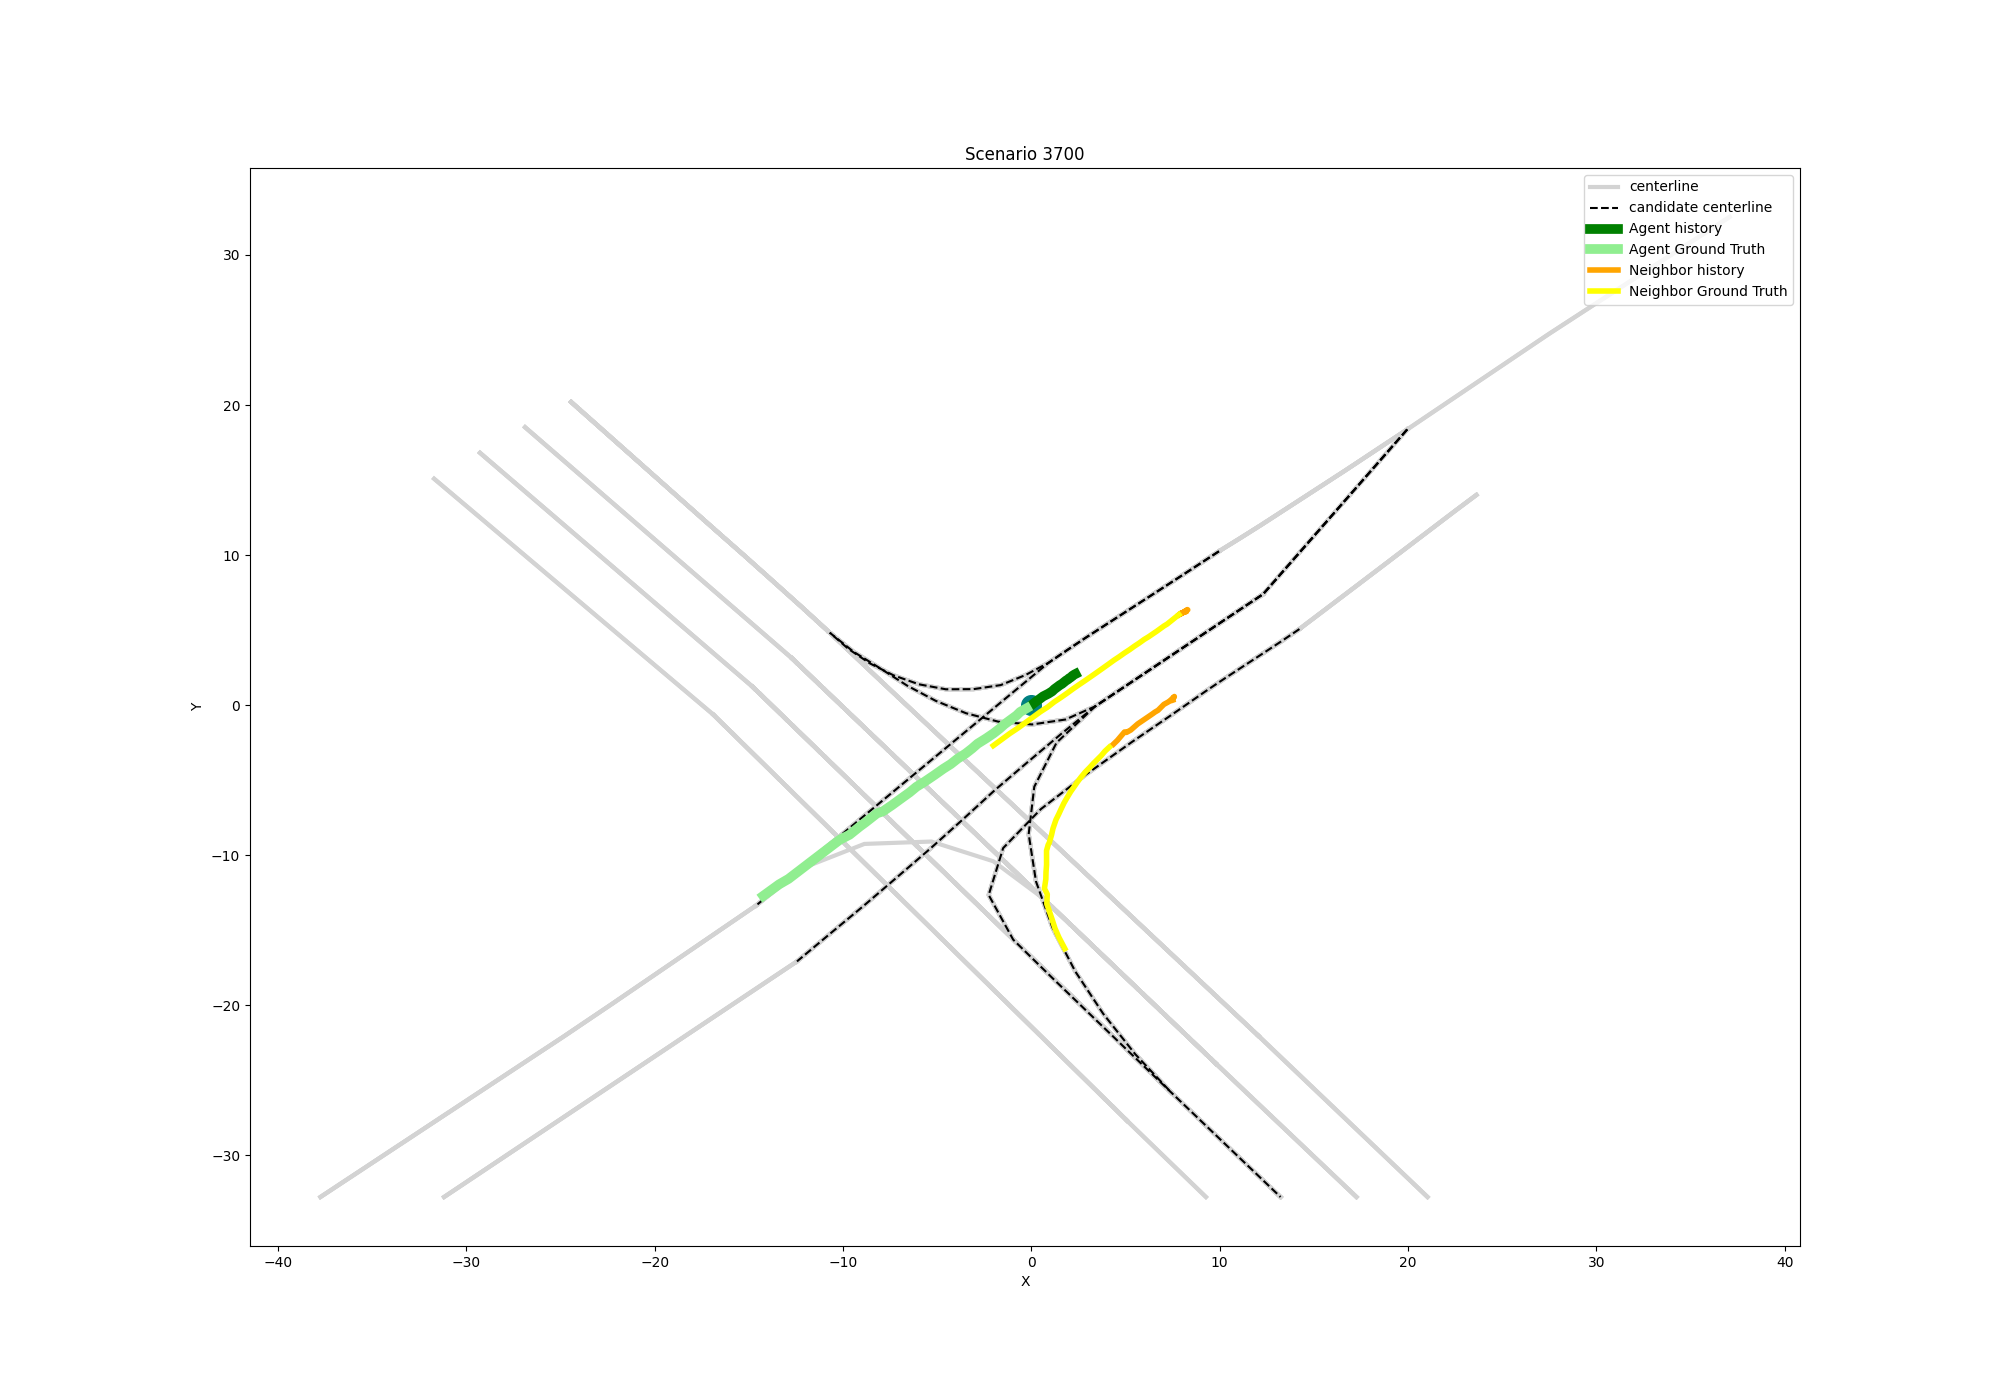
\includegraphics[width=0.9\textwidth]{images/scenario3700.png}
  \caption{Визуализација припремљених података - Пример 1}
  \label{scenario-example-3700}
\end{figure}

\begin{figure}[h!]
  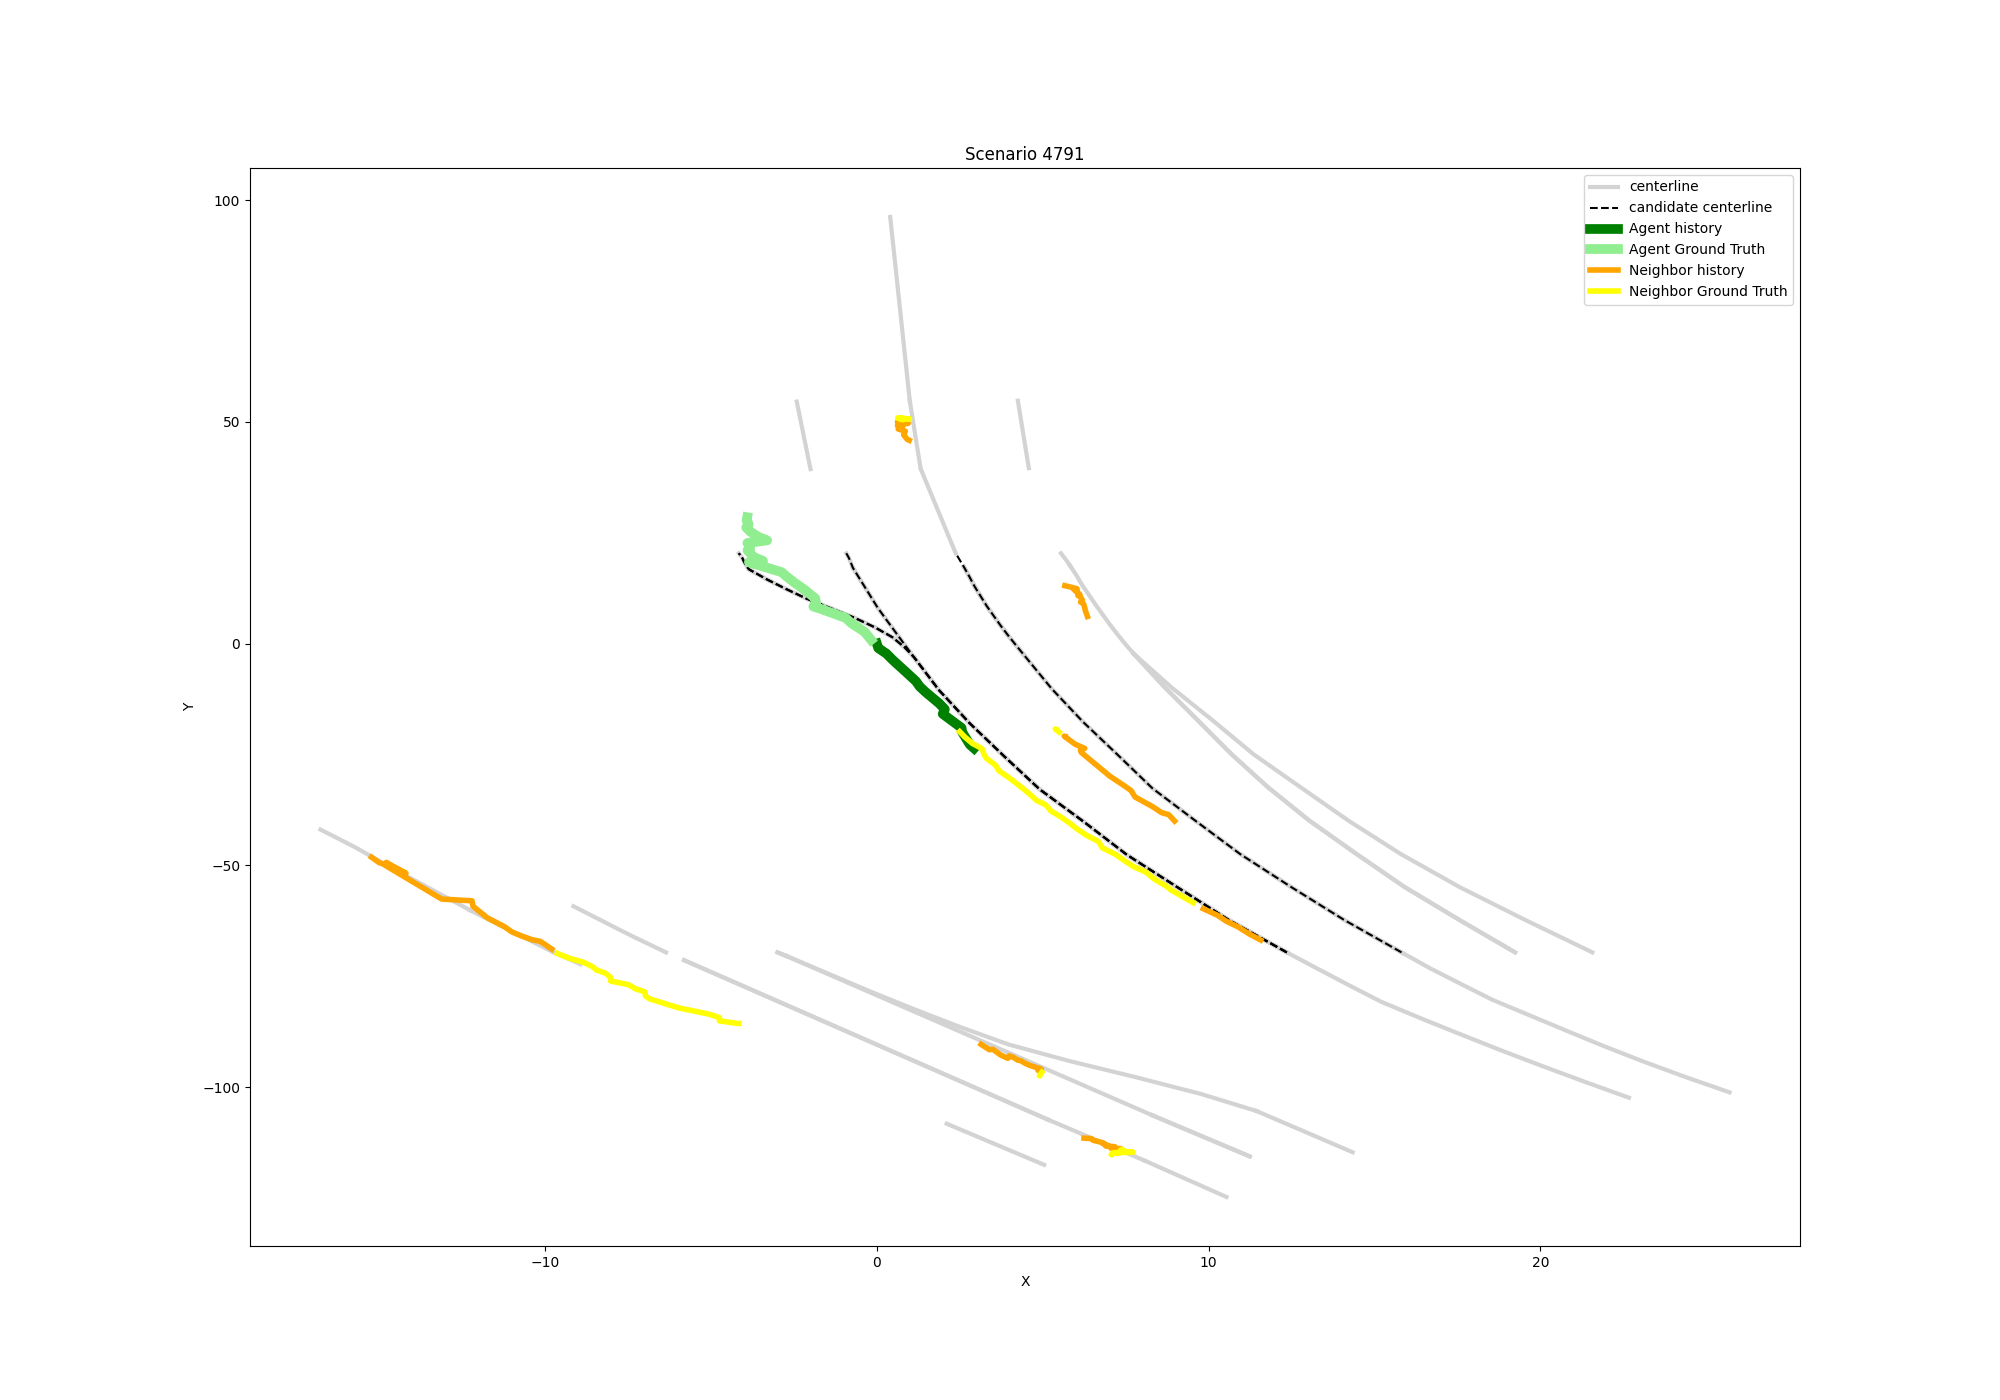
\includegraphics[width=0.9\textwidth]{images/scenario4791.png}
  \caption{Визуализација припремљених података - Пример 2}
  \label{scenario-example-4791}
\end{figure}


% ------------------------------------------------------------------------------
\chapter{Преглед метода за евалуацију модела}
\label{chp:razrada}
% ------------------------------------------------------------------------------

Неке од стандардних метрика за евалуацију квалитета предикције трајекторија су ,,просечнa грешка одступања`` (\textit{eng. ADE - Average Displacement Error})
и ,,последња грешка одступања`` (\textit{eng. FDE - Final Displacement Error}). У наставку се користе енглеске скраћенице \texit{ADE} и
\texit{FDE}. Метрика \textit{ADE} се добија
упросечавањем еуклидског растојања између временски синхронизованих тачака трајекторија предикције и реализације. 
Метрика \textit{FDE} узима у обзир само последњу тачку. \cite{social_gan} \cite{argoverse} 
У наставку се налазе формуле у случају да се посматра тачно један објекат (нпр. само агент):

\begin{figure}[h!]
  \centering
  $ADE = \frac{1}{T}\sum_{k=1}^{T}\sqrt{(x_k - \hat{x}_k)^2 + (y_k - \hat{y}_k)^2}$
\end{figure}

\begin{figure}[h!]
  \centering
  $FDE = \sqrt{(x_{last} - \hat{x}_{last})^2 + (y_{last} - \hat{y}_{last})^2}$
\end{figure}

Метрике се једноставно уопштавају у случајевима где постоји више објеката на сцени:

\begin{figure}[h!]
  \centering
  $ADE = \frac{1}{T\times N}\sum_{n=1}^{N}\sum_{k=1}^{T}\sqrt{(x^n_k - \hat{x}^n_k)^2 + (y^n_k - \hat{y}^n_k)^2}$
\end{figure}

\begin{figure}[h!]
  \centering
  $FDE = \frac{1}{N}\sum_{n=1}^{N}\sqrt{(x^n_{last} - \hat{x}^n_{last})^2 + (y^n_{last} - \hat{y}^n_{last})^2}$
\end{figure}

Ове једноставне метрике су погодне када претпостављамо да је расподела трајекторија унимодална тј. природа трајекторија је претежно детерминистичке. 
Неки скуповима података трајекторија имају јачу стохастичку природу због стохастичке природе самих објеката (трајекторија) или непотпуних опажања окружења. 
Пример таквог скупа података је скуп трајекторија пешака. Пешак који је прешао пешачки прелаз, може у том тренутку да скрене лево или десно.
У том случају имају два вероватна сценарија за исту историју трајекторије (углавном немамо информације о циљевима самог пешака). \cite{social_gan} \cite{best_of_many_cvae}

Скуп ,,најбољи из групе`` (\textit{eng. ,,Best of Many``}) техника узимају у обзир мултимодалну природу расподела трајекторија. Модел може
да генерише неколико различитих предикција трајекторија и за сваку трајекторију одговарајућу вероватноћу (поузданост). Као грешка се узима предикција
која је најбоља по дефинисаном критеријуму (критеријум не мора да се поклапа са самом мером која се користи). \cite{best_of_many_cvae} \cite{argoverse}
Претходно наведене технике \textit{ADE} и \textit{FDE} се уопштавају у \textit{minADE} и \textit{minFDE}. Због једноставности узимају се у обзир облици
са једним објектом: \cite{Disdis} \cite{best_of_many_cvae}

\begin{figure}[h!]
  \centering
  $minADE = ADE(\displaystyle\argmin_{\hat{T}^k_{raj}} FDE(\hat{T}^k_{raj}, T_{raj}), T_{raj}), k \in \{1, ..., K\}$ 
\end{figure}

\begin{figure}[h!]
  \centering
  $minFDE = \displaystyle\min FDE(\hat{T}^k_{raj}, T_{raj}), k \in \{1, ..., K\}$
\end{figure}

Уколико модел генерише више од \texit{K} трајекторија, узима се и обзир првих \texit{K} по поузданости. У специјалном случају када је $K = 1$, онда 
\textit{minFDE} постаје \textit{FDE}, а \texit{minADE} се и даље разликује по избору ,,главне`` трајекторије. 
Проблем са \textit{minADE} i \textit{minFDE} је у томе што не узимају у обзир остале трајекторије поред најбоље и самим тим се не прави разлика
између предикције са свим добрим трајекторијама и предикције са једном добром трајекторијом. \cite{Disdis} 
Друга замерка овим метрикама је што не узимају у обзир поузданост предикција након филтрирања \textit{K} трајекторија. Уколико је најбоља трајекторија
прецизна, желимо и даље да знамо да ли је модел сигуран или је добар резултат последица ,,среће``. Модификоване метрике: \cite{home}

\begin{figure}[h!]
  \centering
  $p\mbox{--}minADE = \sum^T_{k=1} ADE(\hat{T}^{k}_{traj}, T_{raj}) - \ln{P(\hat{T}^{k}_{traj}|E_{nv})}$
\end{figure}

\begin{figure}[h!]
  \centering
  $p\mbox{--}minFDE_{prob} = \sum^T_{k=1} FDE(\hat{T}^{k}_{traj}, T_{raj}) - \ln{P(\hat{T}^{k}_{traj}|E_{nv})}$
\end{figure}

Овде је $p(T^{к}_{traj}|E_{nv})$ условљена вероватноћа те трајекторије у односу на стање окружења. 
Уколико метрика \textit{ADE} (\textit{FDE}) има малу вредност за одговарајућу трајекторију, али њена одговарајућа вероватноћа има малу вредност, 
онда негативан логаритам те вероватноће има велику вредност. \cite{argoverse} У импементацији се ова вероватноћа ограничава са доње стране, како не
би дошло до прекорачења због велике апсолутне вредности након примене логаритма на веома мале вредности.

Уместо упросечавања \textit{L2} растојања у сваком кораку, могу да се броје кораци у којима трајекторије одступају за више од $MR_{thresh}$. 
Мотивација за ову метрику је чињеница да одступање које је 1 или 2 метра од реализације није толико релевантно у односу на 
велику разлику одступања. \cite{home} Такође постоји верзија метрике која узима у обзир вероватноћу и кажњава предикцију 
модела ако је добра, а модел је ипак несигуран.

\begin{figure}[h!]
  \centering
  $MR = \sum^T_{k=1} I(||\hat{T}^{k}_{traj} - T_{raj}||_{2} \geq MR_{thresh})$
\end{figure}

\begin{figure}[h!]
  \centering
  $MR_{prob} = \sum^T_{k=1} I(||\hat{T}^{k}_{traj} - T_{raj}||_{2} \geq MR_{thresh}) $
  $+ I(||\hat{T}^{k}_{traj} - T_{raj}||_{2} < MR_{thresh}) \cdot (1.0 - P(\hat{T}^{k}_{traj}|E_{nv}))$
\end{figure}

\noindent У случају \textit{Argoverse} скупа података, за параметар $MR_{thresh}$ се узима 4 пиксела тј. 2 метра у реалном свету. 

Све до сада наведене метрике су опште примене на било које објекте за које се предвиђају трајекторије. Пошто је агент увек возило, може да
се анализира да ли предикцијa трајекторија скреће са пута. Због тога се уводи метрика ,,сагланост са продучјем вожње`` 
(\textit{eng. DAC - Drivable Area Compilance}), која одређује учесталост трајекторија које нису скренуле са пута од изабраних 
\textit{K} трајекторија: \cite{argoverse}

\begin{figure}[h!]
  \centering
  $DAC = \frac{DAC_{occurences}}{T}$
\end{figure}

У евалуацији модела се узимају у обзир све метрике. За параметар \textit{K} се узима вредност 6.

% ------------------------------------------------------------------------------
\chapter{Техника заснована на разумевању контекста обрадом растеризоване сцене}
\label{chp:razrada}
% ------------------------------------------------------------------------------

У изради...

% ------------------------------------------------------------------------------
\chapter{Техника заснована на разумевању контекста обрадом сцене представљене графом}
\label{chp:razrada}
% ------------------------------------------------------------------------------

У изради...

% ------------------------------------------------------------------------------
\chapter{Евалуација примењених техника}
\label{chp:razrada}
% ------------------------------------------------------------------------------

У изради...

% ------------------------------------------------------------------------------
\chapter{Закључак}
% ------------------------------------------------------------------------------
У изради...

% ------------------------------------------------------------------------------
% Literatura
% ------------------------------------------------------------------------------
\literatura

% ==============================================================================
% Završni deo teze i prilozi
\backmatter
% ==============================================================================

% ------------------------------------------------------------------------------
% Biografija kandidata
\begin{biografija}
\textbf{Момир Аџемовић} 
У изради...
\end{biografija}
% ------------------------------------------------------------------------------

\end{document} 